
前一章中,我們研究了CPU,以及如何使用它們以獲得最佳性能,觀察到CPU有能力並行執行大量指令(指令級並行)。在多個基準測試中看到了CPU可以在每個週期中執行許多操作,而不會造成任何性能損失,例如:添加和減去兩個數字所花費的時間與添加兩個數字所消耗的時間一樣。

但讀者們可能已經注意到,這些基準測試和示例具有一個相當不同尋常的特性。參考以下例子:

\begin{lstlisting}[style=styleCXX]
for (size_t i = 0; i < N; ++i) {
	a1 += p1[i] + p2[i];
	a2 += p1[i] * p2[i];
	a3 += p1[i] << 2;
	a4 += p2[i] – p1[i];
	a5 += (p2[i] << 1)*p2[i];
	a6 += (p2[i] - 3)*p1[i];
}
\end{lstlisting}

這段代碼演示了CPU可以對這兩個值\texttt{p1[i]}和\texttt{p2[i]}進行8次操作,與只進行一次操作的開銷幾乎相同。要非常小心地添加更多的操作,而非添加更多的輸入。某些情況下,只要這些值已經在寄存器中,CPU的內部並行性就會啟用。前面的示例中,在添加第二個、第三個……直到第8個操作時,我們只保留兩個輸入。現實中,對於給定的一組輸入,需要的計算有多少?大多數時候都不到8個。

這並不意味著CPU的計算能力浪費了,除非碰巧運行了前面示例中的奇異代碼。指令級並行性是流水線的計算基礎,流水線可以同時執行循環中不同迭代的操作。無分支計算是用條件指令換取無條件計算,因此可以獲得更多的“不耗時”計算。

然而,問題仍然存在:為什麼要以這種方式限制CPU的基準測試?添加更多輸入,便能夠更輕鬆地輸出8種不同的內容:

\begin{lstlisting}[style=styleCXX]
for (size_t i = 0; i < N; ++i) {
	a1 += p1[i] + p2[i];
	a2 += p3[i] * p4[i];
	a3 += p1[i] << 2;
	a4 += p2[i] - p3[i];
	a5 += (p4[i] << 1)*p2[i];
	a6 += (p3[i] - 3)*p1[i];
}
\end{lstlisting}

這與前面看到的代碼相同,只是現在每次迭代操作4個不同的輸入值,而不是兩個。繼承了前面例子的所有,但僅是因為我們希望在測量某些變化對性能的影響時,儘可能少地進行更改。其對性能的影響還挺大:

%\hspace*{\fill} \\ %插入空行
\begin{center}
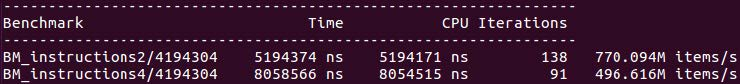
\includegraphics[width=0.9\textwidth]{content/1/chapter4/images/1.jpg}\\
圖 4.1
\end{center}

對4個輸入值進行相同的計算,大約要多花36\%的時間。當需要訪問內存中的數據時,計算就會延遲。

應該注意的是,添加更多的自變量、輸入或輸出可能會影響性能,因為CPU可能正在消耗用於存儲這些變量進行計算的寄存器。雖然這在許多實際的程序中是一個問題,但因為這裡的代碼不夠複雜,不足以佔滿現代CPU的所有寄存器(確認這一點的最簡單方法是檢查機器碼)。

顯然,訪問更多的數據會降低代碼的速度,為什麼呢?高層次的原因是內存跟不上CPU的計算速度。有幾種方法可以估計這種速率的差異,最簡單的方法在現代CPU的參數表中進行查閱。現在的CPU時鐘頻率在3GHz到4GHz之間,一個週期大約是0.3納秒。CPU可以每秒執行幾個操作,所以每納秒執行10個操作並是可能的(儘管在實踐中很難實現,這是一個高效程序的標誌)。另一方面,內存則慢得多,例如:DDR4內存的工作頻率為400Mhz。也可以找到高達3200MHz的值。但這不是內存時鐘,而是數據速率,要將其轉換為類似於內存傳輸數據的速度,還必須考慮\textbf{列訪問頻閃延遲},通常稱為\textbf{CAS延遲}或\textbf{CL}。簡單來說,這是RAM接收數據請求、處理數據並返回值所需的週期數。沒有在所有情況下都有意義的內存速度定義(本章後面,我們將看到原因),但是,對於數據速率為3.2GHz和CAS延遲15的DDR4模塊來說,其內存速度大約是107MHz,即每次訪問9.4需要納秒。

無論從哪個角度來看,CPU每秒執行的操作要比內存為這些操作提供輸入值或存儲結果的能力強。程序需要以某種方式使用內存,訪問內存的細節將對性能產生重大影響,有時甚至會限制內存。然而,內存速率差對性能的影響會從微不足道到實際瓶頸。所以,必須瞭解不同條件下的內存如何影響程序性能,以及原因是什麼,這樣就可以利用這些知識來設計和優化自己的代碼,從而獲得最佳性能。








